\documentclass{beamer}

%\usetheme{AnnArbor}
\usetheme{Warsaw}
\usecolortheme{seahorse}
\usecolortheme{rose}
\usefonttheme[onlylarge]{structuresmallcapsserif}
\usefonttheme[onlysmall]{structurebold}
\setbeamerfont{title}{shape=\itshape,family=\rmfamily}
%\setbeamercolor{title}{fg=red!80!black}

\usepackage{caption}
\usepackage{subcaption}
%\usecolortheme{wolverine}
\usepackage[utf8]{inputenc}
\usepackage[T1]{fontenc}
\usepackage[french]{babel}
\usepackage{tikz}
\usepackage{animate}
%\usepackage{graphicx}
\usepackage{blkarray}
\usepackage{graphicx}

\title{TRON GAME}
\author[A. Catherine ATTY \\  Sékou DOUMBOUYA \\ Manne Emile KITSOUKOU \\ Amirath Fara OROU-GUIDOU]{A. Catherine ATTY \\  Sékou DOUMBOUYA \\ Manne Emile KITSOUKOU \\ Amirath Fara OROU-GUIDOU}
\institute[Université de Caen Normandie]{Université de Caen Normandie}
\date{\today}
\logo{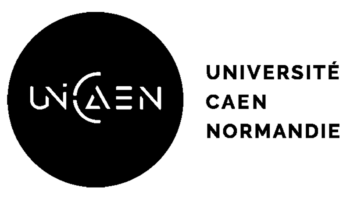
\includegraphics[width=0.2\textwidth]{Images/universite-de-caen-normandie-1-350x0-c-default.png}}

\setbeamertemplate{footline}[frame number]

\begin{document}
    % page de garde
    \begin{frame}
        \titlepage
    \end{frame}
    
    \section*{Introduction}
    \subsection*{Objectifs et Enjeux du projet}

    % Objectifs du projet
    \begin{frame}{Objectifs du projet}
        \begin{block}{Ce projet avait pour objectif de :}
            \begin{itemize}
                \item Modélisation du jeu
                \item Mise en place d'une interface graphique
                \item Implémentation et optimisation des algorithmes de recherche
                \item Analyser et comparer les performances des algorithmes Maxn et paranoid
            \end{itemize}
        \end{block}
    \end{frame}

    % Enjeux du projet
    \begin{frame}{Enjeux du projet}
        \begin{block}{Les enjeux qu'il a fallu relever :}
            \begin{itemize}
                \item Evaluation de l'efficacité de différentes approches algorithmiques 
                \item Identification des paramètres influant sur les performances des algorithmes
                \item Comprendre les mécanismes de prise de décision
            \end{itemize}
        \end{block}
    \end{frame}

\subsection*{Plan du projet}
    % Plan du projet
    \begin{frame}{Plan du projet}
        \tableofcontents
    \end{frame}

    \section{Conception du jeu de TRON}
    \subsection*{Modélisation du jeu}
    % Modélisation du jeu
    \begin{frame}{Modélisation du jeu}
        \begin{block}{Les principaux éléments du jeu sont :}
            \begin{itemize}
                \item \textbf{Player} : représente un joueur
                \item \textbf{Move} : structure les données d'un mouvement
                \item \textbf{Board} : modelise le plateau de jeu
                \item \textbf{State} : représente l'état du jeu
            \end{itemize}
        \end{block}
        \begin{figure}
            \begin{center}
                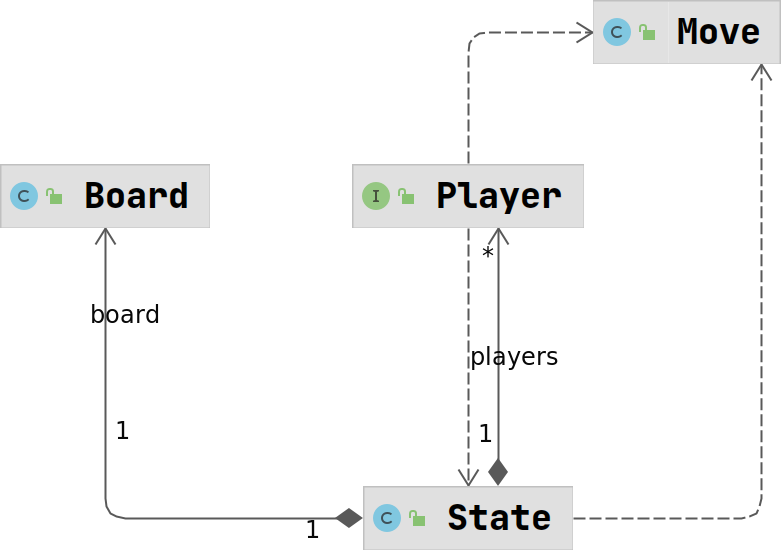
\includegraphics[scale=0.25]{Images/model}
                \caption{Modélisation du jeu}
            \end{center}
        \end{figure}
    \end{frame}

% Interface graphique
\subsection*{Interface graphique}
    % Interface graphique
    \begin{frame}{Mise en place d'une interface graphique}
        \begin{figure}
            \begin{center}
                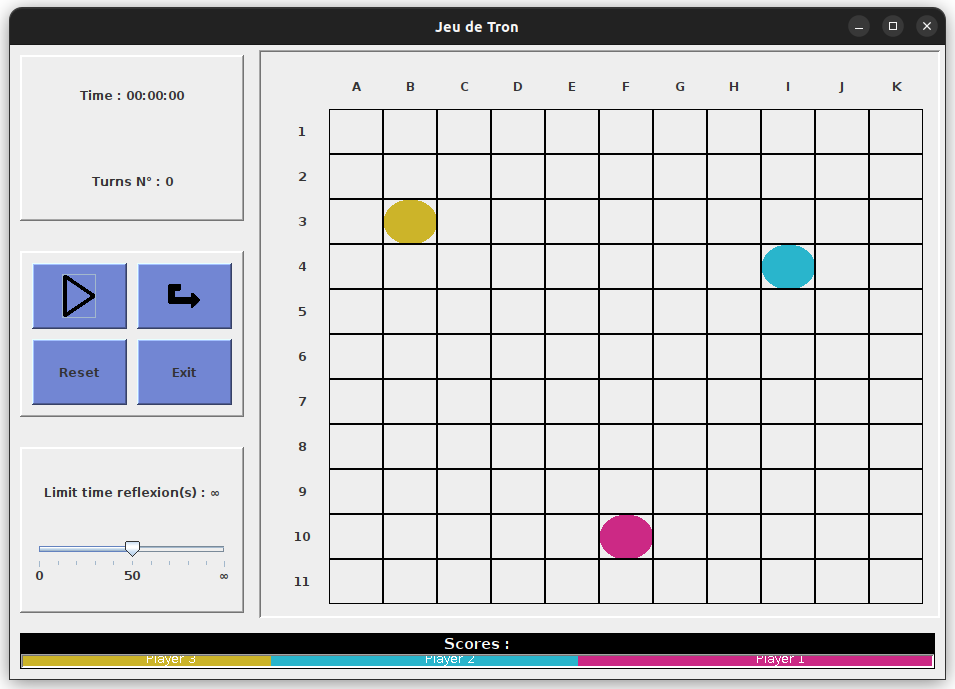
\includegraphics[scale=0.25]{Images/fenetrejeu}
                \caption{Interface graphique}
            \end{center}
        \end{figure}
    \end{frame}

% Fonctionnalités de l'interface graphique
\subsection*{Fonctionnalités}
    % Fonctionnalités de l'interface graphique
    \begin{frame}{Fonctionnalités interface graphique}
        \begin{block}{On peut principalement :}
            \begin{itemize}
                \item \textbf{Lancer une partie} : lancer une partie avec les paramètres choisis
                \item \textbf{Rejouer une partie} : rejouer une partie déjà jouée
                \item \textbf{Changer les paramètres} : changer les paramètres de la partie
            \end{itemize}
        \end{block}
    \end{frame}





    \section{Heuristiques et Analyse}
    \begin{frame}{Heuristiques}
    \centering
    \Large \textbf{Comment choisir le meilleur coup ?}
\end{frame}

\begin{frame}{Heuristiques}
    \begin{block}{Définition}
        \begin{itemize}
            \item Une heuristique est une fonction qui permet de déterminer la valeur d'un état du jeu
            \item Elle est utilisée pour choisir le meilleur coup à jouer
        \end{itemize}
    \end{block}
\end{frame}

% On liste les heuristiques utilisées
\subsection*{Présentation des Heuristiques}
    % Présentation des heuristiques
    \begin{frame}{Présentation des heuristiques}
        \begin{block}{On a utilisé les heuristiques suivantes :}
            \begin{itemize}
                \item \textbf{OpenSpace}
                \item \textbf{GSALAP}
                \item \textbf{Voronoi}
                \item \textbf{Checker}
            \end{itemize}
        \end{block}
    \end{frame}

    % On présente l'heuristique OpenSpace
    \begin{frame}{OpenSpace}
        \begin{block}{Description}
            \begin{itemize}
                \item On compte le nombre de cases vides autour de la case où on veut jouer
                \item On choisit le coup qui maximise ce nombre
            \end{itemize}
            % On rajoutera une image
            \begin{figure}
                \begin{center}
                    \includegraphics[scale=0.25]{Images/OpenSpace.png}
                    \caption{OpenSpace}
                \end{center}
            \end{figure}
        \end{block}
    \end{frame}

    % On présente l'heuristique GSALAP
    \begin{frame}{GSALAP}
        \begin{block}{GSALAP ou \textit{Go AS Long As Possible}}
            \begin{itemize}
                \item On compte le nombre de pions qu'on peut jouer avant de bloquer
                \item On choisir le coup qui maximise ce nombre
            \end{itemize}
        \end{block}
        \begin{figure}
            \begin{center}
                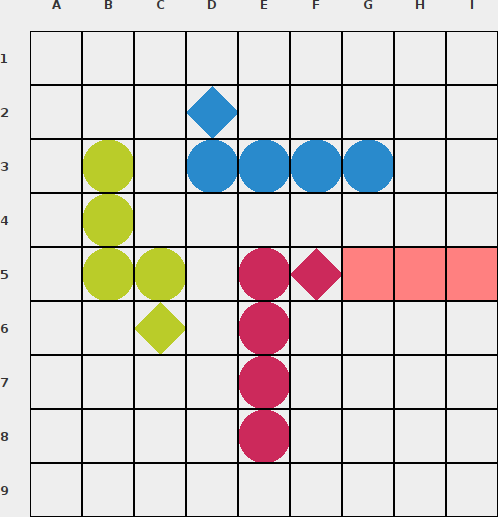
\includegraphics[scale=0.25]{Images/GSLASP.png}
                \caption{GSALAP}
            \end{center}
        \end{figure}
    \end{frame}

    % On présente l'heuristique Voronoi
    \begin{frame}{Voronoi}
        \begin{block}{Description}
            \begin{itemize}
                \item On détermine la distance entre chaque case vide et la tête de chaque joueur
                \item On choisit le coup qui maximise la distance entre la tête du joueur et la case vide
            \end{itemize}
            % On rajoutera une image
            \begin{figure}
                \begin{center}
                    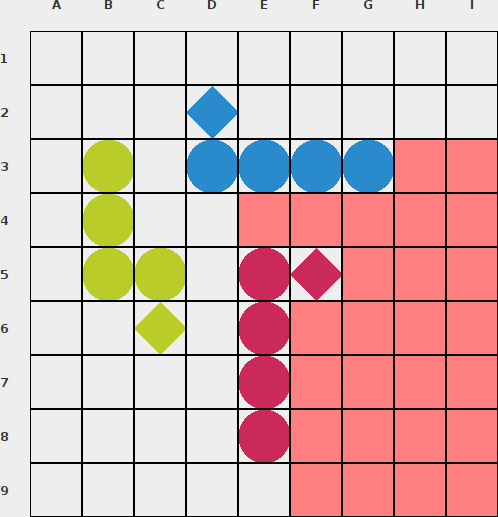
\includegraphics[scale=0.25]{Images/Voronoi.png}
                    \caption{Voronoi}
                \end{center}
            \end{figure}
        \end{block}
    \end{frame}

    % On présente l'heuristique Checker
    \begin{frame}{Checker}
        \begin{block}{Description}
            \begin{itemize}
                \item On compte le nombre de cases vides autour de la case où on veut jouer
                \item On choisit le coup qui maximise ce nombre
            \end{itemize}
            % On rajoutera une image
        \end{block}
    \end{frame}

    % Complexité des heuristiques
    \subsection*{Complexité des heuristiques}
    \begin{frame}{Complexité des heuristiques}
        \begin{block}{Complexité en temps des heuristiques :}
            \begin{table}[]
                \begin{tabular}{|l|l|}
                \hline
                                            & \textbf{Complexité en temps}               \\ \hline
                \textit{\textbf{OpenSpace}} & $\mathcal{O}(J)$                           \\ \hline
                \textit{\textbf{GSLASP}}    & $\mathcal{O}(J \times N)$                  \\ \hline
                \textit{\textbf{Voronoï}}   & $\mathcal{O}{(J(|A| + |S|log|S|) + |S|J)}$ \\ \hline
                \textit{\textbf{Checker}}   & $\mathcal{O}{(J(|A| + |S|log|S|) + |S|J)}$ \\ \hline
                \end{tabular}
                \end{table}
        \end{block}
    \end{frame}

    \subsection*{Comparaison des heuristiques}
    \begin{frame}{Performances des heuristiques avec \textbf{\texttt{Max$^n$}}}
        % On met les 2 figures cotes à cotes
        \begin{columns}
            \begin{column}{0.5\textwidth}
                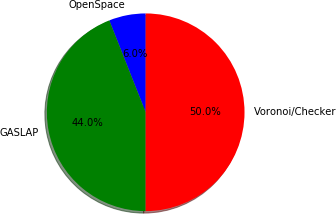
\includegraphics[scale=0.5]{Images/ProporitionVictoireHeuristiqueWithMaxN.png}
                \captionof{figure}{Victoire par heuristique}
            \end{column}
            \begin{column}{0.5\textwidth}
                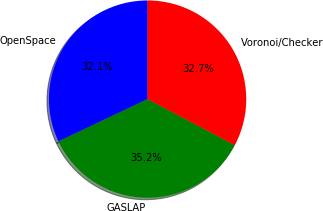
\includegraphics[scale=0.5]{Images/ProportionDureePartieGagnanteWithMaxN.png}
                \captionof{figure}{Durée des parties gagnantes}
            \end{column}
        \end{columns}
    \end{frame}

    \begin{frame}{Performances des heuristiques avec \textbf{\texttt{Max$^n$}}}
        \begin{columns}
            \begin{column}{0.5\textwidth}
                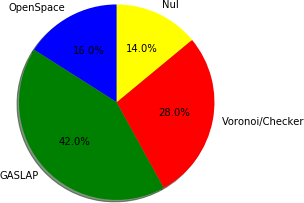
\includegraphics[scale=0.5]{Images/ProporitionVictoireHeuristiqueWithParanoid.png}
                \captionof{figure}{Victoire par heuristique}
            \end{column}
            \begin{column}{0.5\textwidth}
                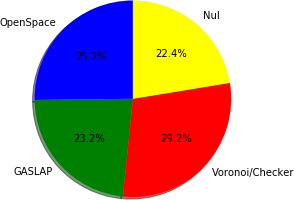
\includegraphics[scale=0.5]{Images/ProportionDureePartieGagnanteWithParanoid.png}
                \captionof{figure}{Durée des parties gagnantes}
            \end{column}
        \end{columns}
    \end{frame}





    \section{Étude des performances}
    \begin{frame}
    
\end{frame}

    \section{Conclusion}
    \begin{frame}
    
\end{frame}

\end{document}
ï